\documentclass[german]{latex4ei/latex4ei_sheet}





\begin{document}

\section{Wellen und Leitungen}
\begin{sectionbox}
\begin{itemize}
    \item Maxwellgleichungen
    \item Physikalisch relevante partielle Differentialgleichungen (Potentialgleichung,
        Diffusionsgleichung, Wellengleichung)
    \item Schnell veränderliche elektromagnetische Felder, Wellenausbreitung
    \item Ebene Wellen, harmonische Wellen, polarisierte Wellen, Poynting-Vektor
    \item Wellengleichung in reeller, komplexer und Phasorendarstellung
    \item Reflexion und Transmission elektromagnetischer Wellen an Grenzflächen
    \ verlustlose Leitungstheorie: Leitungsarten, Pulse auf Leitungen, Impedanz, Anpassung
    \item verlustbehaftete Leitungstheorie: Dispersion, Phasen- und Gruppengeschwindigkeit
    \item Antennen, Nahfeld, Fernfeld
\end{itemize}

\end{sectionbox}


\section{Formelzeichen}
\begin{sectionbox}
    \begin{itemize}
        \item $\nabla = $ Nabla-Operator
        \item $\Delta = \nabla^2 = $ Laplace-Operator
        \item $\vec{E} = $ elektrische Feldstärke
        \item $\vec{B} = \mu \vec{H} = \mathbf{rot}\vec{A}$ magnetische Flussdichte
        \item $\vec{H} = $ magnetische Feldstärke
        \item $\vec{D} = \varepsilon \vec{E}$ elektrische (Verschiebungs-) Flussdichte
        \item $\vec{S} = \vec{g} = \vec{J} = \kappa \vec{E}   $ Stromdichte
        \item $\rho = $ Ladungsdichte
        \item $\varepsilon = \varepsilon_0 \cdot \varepsilon_r= $ (elektrische) Permittivität
        \item $ \mu = \mu_0 \cdot \mu_r = $ (magnetische) Permeabilität
        \item $ \kappa = \sigma = $ el. Leitfähigkeit (bestimmt Verluste)
        \item $\phi = $ elektrisches Potential
        \item $\vec{A} = $ magnetisches Vektorpotential
        \item $\tau = $ Volumenelement
        \item $\Phi = $ magnetischer Fluss
        \item $\Psi = $ elektrischer Fluss
        \item $I = $ Stromstärke
        \item $Q = $ Ladung
    \end{itemize}
\end{sectionbox}

\section{Skalar- und Vektorfelder}
\begin{sectionbox}
    \textbf{Skalarfeld:} $f: \mathbb{R}^n \to \mathbb{R}$\\
    Jedem Punkt im Raum ist ein Skalar zugeordnet.\\
    Beispiel: Temperaturverteilung in einem Raum.\\

    \textbf{Vektorfeld:} $\vec{f}: \mathbb{R}^n \to \mathbb{R}^m$\\
    Jedem Punkt im Raum ist ein Vektor zugeordnet.\\
    Beispiel: Windgeschwindigkeit in einem Raum.\\

    \textbf{Gradientenfeld:} $\nabla f = \left( \frac{\partial f}{\partial x_1}, \frac{\partial f}{\partial x_2}, \ldots, \frac{\partial f}{\partial x_n} \right)$\\
    Der Gradient eines Skalarfeldes ist ein Vektorfeld.\\
    Der Gradient zeigt in die Richtung des steilsten Anstiegs des Skalarfeldes.\\

    \textbf{Divergenzfeld:} $\nabla \bullet \vec{f} = \frac{\partial f_1}{\partial x_1} + \frac{\partial f_2}{\partial x_2} + \ldots + \frac{\partial f_m}{\partial x_m}$\\
    Die Divergenz eines Vektorfeldes ist ein Skalarfeld.\\
    Die Divergenz misst die Quellenstärke eines Vektorfeldes.\\

    \textbf{Rotationsfeld:} $\nabla \times \vec{f} = \left( \frac{\partial f_3}{\partial x_2} - \frac{\partial f_2}{\partial x_3}, \frac{\partial f_1}{\partial x_3} - \frac{\partial f_3}{\partial x_1}, \frac{\partial f_2}{\partial x_1} - \frac{\partial f_1}{\partial x_2} \right)$\\
    Die Rotation eines Vektorfeldes ist ein Vektorfeld.\\
    Die Rotation misst die Wirbelstärke eines Vektorfeldes.\\

    \textbf{Besondere Felder:}
    \begin{itemize}
        \item \textbf{Quellenfreies Feld:} $\nabla \bullet \vec{f} = 0$\\
        Ein divergenzfreies Feld hat keine Quellen.\\
        Beispiel: Magnetfeld
        \item \textbf{Konservatives Feld:} $\nabla \times \vec{f} = 0$\\
        Ein konservatives oder wirbelfreies Feld hat keine Wirbel.\\
        Wegunabhängige Integrale.\\
        Beispiel: Elektrostatisches Feld, Gravitationsfeld \\
    \end{itemize}

\end{sectionbox}


\begin{sectionbox}
    \textbf{Satz von Stokes:}\\
    Sei $A$ eine orientierte Fläche mit Rand $\vec{s}$. Dann gilt:
    \begin{equation*}
        \int_{A} \mathbf{rot}\vec{f} \cdot d\vec{A} = \oint  \vec{f} \cdot d\vec{s}
    \end{equation*}
    Der Satz von Stokes verknüpft die Linienintegrale entlang des Randes einer Fläche mit dem Flächenintegral über die Rotation des Vektorfeldes über der Fläche.\\

    \textbf{Satz von Gauß:}\\
    Sei $V$ ein Volumen mit Hülle $A$. Dann gilt:
    \begin{equation*}
        \int_{V} \mathbf{div}\vec{f} \cdot d\tau = \oint_{A} \vec{f} \cdot d\vec{A}
    \end{equation*}
    Der Satz von Gauß verknüpft die Flächenintegrale entlang der Randfläche eines Volumens mit dem Volumenintegral über die Divergenz des Vektorfeldes über dem Volumen.\\
\end{sectionbox}

\section{Eektro- und Magnetostatik}
\begin{sectionbox}
    Ladungen verursachen Quellen des elektrischen Feldes,
    Ströme Wirbel des magnetischen Feldes. \\

    \textbf{Elektrostatik:}\\
    \textbf{E-Feld:} $\vec{E} = -\grad \phi = -\nabla \phi$\\
    Der Gradient des elektrischen Potentials $\phi$ ergibt das elektrische Feld $\vec{E}$.\\

    \subsubsection{Strömungsfelder}
    \textbf{Durchflutungsgesetz:}\\
    mit $\mathbf{rot}\vec{H} = \vec{g}$
    \begin{equation*}
        I = \oint \vec{H} \cdot d \vec{s} = \int_{A} \mathbf{rot}\vec{H} \cdot d \vec{A} =\int_{A} \vec{g} \cdot d \vec{A}
    \end{equation*}
\end{sectionbox}

\section{Maxwell-Gleichungen}
\begin{sectionbox}
    \textbf{Maxwell-Gleichungen differentiell:}\\
    \begin{itemize}
        \item \textbf{1. Maxwell-Gleichung:} $\mathbf{div}\vec{E} = \nabla \bullet \vec{E} = \frac{\rho}{\varepsilon_0}$\\
              Die Divergenz (Quellendichte) des elektrischen Feldes ist proportional zur Ladungsdichte.\\  
        \item \textbf{2. Maxwell-Gleichung:} $\nabla \bullet \vec{B} = 0$\\
                Die Divergenz (Quellendichte) des magnetischen Feldes ist null.\\
                Es gibt keine magnetischen Monopole.\\
        \item \textbf{3. Maxwell-Gleichung:} $\nabla \times \vec{E} = -\frac{\partial \vec{B}}{\partial t}$ \vspace{1mm}\\
              Oder auch Induktionsgesetz von Faraday besagt, dass die zeitliche Veränderung einer Flussdichte ein rotierendes E-Feld erzeugt.\\
              In einem geschlossenen Stromkreis wird eine Spannung induziert, wenn sich der magnetische Fluss ändert.\\
        \item \textbf{4. Maxwell-Gleichung:} $\nabla \times \vec{B} = \mu_0\vec{j} + \mu_0\varepsilon_0\frac{\partial \vec{E}}{\partial t}$\vspace{1mm}\\
                Oder auch Ampere-Maxwell-Gesetz besagt, dass die Rotation eines magnetischen Feldes proportional zur Summe aus elektrischem Strom und der Veränderung der el. Verschiebungsflussdichte ist.\\
    \end{itemize}
    Die Maxwell-Gleichungen beschreiben die Wechselwirkungen zwischen elektrischen und magnetischen Feldern.\\

    \textbf{Maxwell-Gleichungen integral:}\\
    \begin{itemize}
        \item \textbf{1. Maxwell-Gleichung:} $\oint \vec{E} \cdot d\vec{A} = \frac{Q}{\varepsilon_0}$\\
        \item \textbf{2. Maxwell-Gleichung:} $\oint \vec{B} \cdot d\vec{A} = 0$\\
        \item \textbf{3. Maxwell-Gleichung:} $\oint \vec{E} \cdot d\vec{s} = -\dot{\Phi} = -\frac{\partial}{\partial t}\int_{A}\vec{B} \cdot d\vec{A}$\\
        \item \textbf{4. Maxwell-Gleichung:} $\oint \vec{B} \cdot d\vec{s} = \mu_0 I + \mu_0\varepsilon_0\frac{\partial}{\partial t}\int_{A}\vec{E} \cdot d\vec{A}$\\
    \end{itemize}
\end{sectionbox}


\section{Wichtige Differentialgleichungen}
\begin{sectionbox}
    \textbf{Poisson-Gleichung:}\\
    \begin{equation*}
        \Delta \phi = -\frac{\rho}{\varepsilon_0}
    \end{equation*}
    Die Verteilung der Ladungsdichte $\rho$ entspricht der Quellenstärke eines el. Feldes.
    Das el. Feld entspricht dem Gefälle einer Potentialverteilung (Gradient). Die Ladungsdichte ist also proportional zur Krümmung der Potentialverteilung.\vspace{2mm} \\
    \textbf{Diffusionsgleichung:}\\
    \begin{equation*}
        \Delta f = \mu \kappa \frac{\partial f}{\partial t}
    \end{equation*}
    Die Geschwindigkeit der Diffusion eines Feldes $f = \vec{E}, \vec{S}, \vec{B}, \vec{A}$ ist proportional zur Krümmung seiner Feldstärke .\vspace{2mm}\\
    \textbf{spezielle Wellen-Gleichungen:}\\
    \begin{equation*}
        c^2 \Delta \vec{E} = \frac{\partial^2 \vec{E}}{\partial t^2}  \hspace{10mm}  c^2 \Delta \vec{B} = \frac{\partial^2 \vec{B}}{\partial t^2}
    \end{equation*}
    Die Änderung der Geschwindigkeit der Feldstärkenänderung ist proportional zur Änderungsrate der Steigung eines Gefälles oder auch Krümmung in der Feldstärke.\\
    vgl. sin/cos Funktion: maximale Krümmung $\rightarrow$ minimale Änderungsgeschwindigkeit $\rightarrow$ maximale Änderung der Änderungsgeschwindigkeit\\
\end{sectionbox}



\begin{sectionbox}
    \textbf{Relaxationszeit:} $t_r = \frac{\varepsilon}{\kappa}$ \vspace{1mm}\\
    \textbf{Abschätzungen der Diffusionszeit:}
    \begin{equation*}
        t_0 \approx \mu \kappa l^2
    \end{equation*}
    Mit $t_0$ als Diffusionszeit (vollständige durchdringung) und $l$ der küzesten Strecke durch den Körper in Diffusionsrichtung. \vspace{2mm}\\
    \textbf{Abschätzung Eindringtife Leiter im Wechselfeld:}
    \begin{equation*}
        l \approx \frac{1}{\sqrt{\omega \mu \kappa}} 
    \end{equation*}

    \textbf{Grenzfall $\Omega \ll 0$:} Stromdichte räumlich konstant, zeitlich langsam oszillierend.\\
    \textbf{Grenzfall $\Omega \gg 0$:} Wie ebene Diffusion im Halbraum.\\
\end{sectionbox}


\section{Elektromagnetische Wellen}
\begin{sectionbox}
    \textbf{Harmonische ebene Welle:} (Ausbreitung in $z$-Richtung / Nichtleiter) \\
    \[
    \begin{aligned}
        & E_x(z, t) = E_{x0} \cos(\omega t - kz + \varphi), \\
        & H_y(z, t) = H_{y0} \cos(\omega t - kz + \varphi), \\
        & H_{y0} = \frac{E_{x0}}{Z}
    \end{aligned}
    \]
    \begin{itemize}
        \item Wellenlänge: $\lambda = \frac{c}{f}$ \vspace{1mm}
        \item Frequenz: $f = \frac{1}{T}$ \vspace{1mm}
        \item Kreisfrequenz: $\omega(k) = 2\pi f = \frac{2\pi c}{\lambda} = ck$ \vspace{1mm}
        \item Wellenzahl: $k = \frac{2\pi}{\lambda} = \frac{\omega}{c}$ \vspace{1mm}
        \item Phasengeschwindigkeit: $c = \frac{1}{\sqrt{\varepsilon \mu}} = \frac{\omega(k)}{k}$ \vspace{1mm}
        \item Gruppengeschwindigkeit: $v_g = \frac{\partial \omega(k)}{\partial k}$ \vspace{1mm}
        %\item Energie: $E = hf$\\
        %\item Impuls: $p = \frac{h}{\lambda}$\\
        \item Wellenwiderstand: $Z = \frac{E}{H} = \sqrt{\frac{\mu}{\varepsilon}}$ \hspace{5mm} Im Vakuum $= 377 \Omega$ \vspace{1mm}
        \item elliptische Polarisation: \\ $E = E_{y0} \cos(\omega t - kz) E_{x0} \cos(\omega t - kz + \varphi)$ \vspace{1mm}
        \item TE- (H-) Welle: Longitudinalkomponente im H-Feld und andersrum.
    \end{itemize}
    

\end{sectionbox}


\begin{sectionbox}
    \textbf{Analogie zu Strom und Spannung:}\\
    Widerstand $R = \frac{U}{I}$\\
    Wellenwiderstand $Z = \frac{E}{H}$ (Nur bei Phasengleichheit im Fernfeld)\\
    $$Z = \sqrt{\frac{\mu}{\varepsilon}}$$\\
    \textbf{Energie}\\
    \textbf{Poynting-Vektor:} $\vec{S} = \vec{E} \times \vec{B} = (0,0,E_xH_y) = \left(0,0, \dfrac{E_x^2}{Z}\right)$\\
    zeitlich gemittelt: $\bar{|\vec{S}|} = \frac{E_{eff}^2}{Z_0}$ \hspace{3mm} mit \hspace{3mm} $E_{eff} = \frac{\hat{E}}{\sqrt{2}}$\\
    TE-Welle: $\vec{S} = (0,-E_xH_z,E_xH_y)$
    
\end{sectionbox}

\subsection{Hertzscher Dipol}
\begin{sectionbox}
    Der Hertzsche Dipol entspricht einem oszillierenden elektrischen Dipol, der
    über das Stromelement periodisch umgeladen wird. \\

    Das Feld lässt sich aus der dem Potential oder der überlagerung infinitesimaler Stromelemente berechnen. \\
    \[
\vec{A}(\mathbf{r}) = \frac{\mu}{4 \pi} \iiint \frac{\vec{J}(\vec{r}') e^{-j k |\vec{r} - \vec{r}'|}}{|\vec{r} - \vec{r}'|} \, \mathrm{d}V'
\]
\[
\vec{E} = -j \omega \left( 1 + \frac{1}{k^2} \, \mathbf{grad} \, \mathbf{div} \right) \vec{A}
\]



\begin{align*}
E_r &= \frac{I l}{2 \pi} k^2 Z \cos\theta \left( \frac{1}{(kr)^2} - j \frac{1}{(kr)^3} \right) e^{-jkr}, \\
E_\theta &= \frac{I l}{4 \pi} k^2 Z \sin\theta \left( j \frac{1}{(kr)} + \frac{1}{(kr)^2} - j \frac{1}{(kr)^3} \right) e^{-jkr}, \\
H_\phi &= \frac{I l}{4 \pi} k^2 \sin\theta \left( j \frac{1}{(kr)} + \frac{1}{(kr)^2} \right) e^{-jkr}
\end{align*}


    \textbf{Nahfeld:}\\ 
    Das Nahfeld des Hertzschen Dipols ist ein kapazitives, hochohmiges Feld,
    indem das elektrische Feld dem magnetischen um 90° nacheilt.
    \[
        \text{für} \hspace{5mm} kr = 2 \pi \frac{r}{\lambda} \ll 1 \hspace{5mm} \text{gilt} \hspace{5mm} \frac{1}{(kr)^3} \gg \frac{1}{(kr)^2} \gg \frac{1}{(kr)}
    \]

    \textbf{Fernfeld:}\\
    Im Fernfeld des Hertzschen Dipols sind elektrisches und magnetisches Feld
    zeitlich in Phase und transversal zur Ausbreitungsrichtung (TEM-Feld).
    \[
        \text{für} \hspace{5mm} kr = 2 \pi \frac{r}{\lambda} \gg 1 \hspace{5mm} \text{gilt} \hspace{5mm} \frac{1}{(kr)} \gg \frac{1}{(kr)^2} \gg \frac{1}{(kr)^3}
    \]
    \textbf{Strahlungswiderstand/Leistung:}\\
    \[
        P_r = \frac{|I|^2}{2} \cdot R_r \hspace{5mm}  \text{mit} \hspace{5mm} R_r =  \frac{2 \pi}{3} Z \left(\frac{l}{\lambda}\right)^2
    \]

\end{sectionbox}

\subsection{Reflexion und Brechung ebener Wellen}
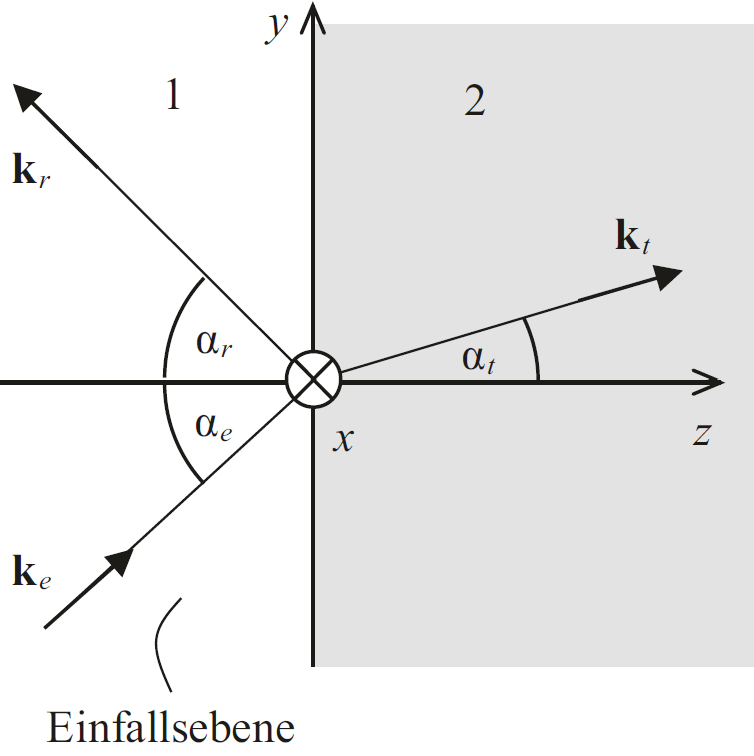
\includegraphics[width = \columnwidth]{images/einfallswinkel.png}
\begin{sectionbox}
    \textbf{Senkrechte Polarisation:}\\
    (der E-Vektor ist in der Einfallsebene)\\
    \begin{equation*}
        r_s = \frac{Z_2 \cos \alpha_1 - Z_1 \cos \alpha_2}{Z_2 \cos \alpha_1 + Z_1 \cos \alpha_2} \hspace{5mm} t_s = \frac{2 Z_2 \cos \alpha_1}{Z_2 \cos \alpha_1 + Z_1 \cos \alpha_2}
    \end{equation*}	
    \textbf{Parallelpolarisation:}\\
    (der E-Vektor ist senkrecht zur Einfallsebene)\\
    \begin{equation*}
        r_p = \frac{Z_1 \cos \alpha_1 - Z_2 \cos \alpha_2}{Z_1 \cos \alpha_1 + Z_2 \cos \alpha_2} \hspace{5mm} t_p = \frac{2 Z_2 \cos \alpha_1}{Z_1 \cos \alpha_1 + Z_2 \cos \alpha_2} 
    \end{equation*}
\end{sectionbox}


\section{Leitungen}
\begin{sectionbox}
    \textbf{Allgemeine Wellengleichungen:}\\
    (Herleitung mit Identität $\mathbf{rot} \hspace{1mm} \mathbf{rot} \vec{A} = \mathbf{grad} \hspace{1mm} \mathbf{div}\vec{A} - \Delta \vec{A}$)
    \begin{equation*}
        \begin{aligned}
            &\Delta \vec{E} - \mathbf{grad} \hspace{1mm} \mathbf{div} \vec{E} = \mu \kappa \frac{\partial \vec{E}}{\partial t} + \mu \varepsilon \frac{\partial^2 \vec{E}}{\partial t^2}\\
            &\Delta \vec{B} = \mu \kappa \frac{\partial \vec{B}}{\partial t}+ \mu \varepsilon \frac{\partial^2 \vec{B}}{\partial t^2}
        \end{aligned}
    \end{equation*}

    \textbf{Komplexe Wellenarstellung}\\
    (Mit Wellenzahlvektor $\vec{k}$  zum Zeitpunkt $t$ am Punkt $\vec{r}$):
    \begin{equation*}
            \vec{E} = E_0 e^{j(\omega t - \vec{k} \cdot \vec{r})} \hspace{10mm} \vec{B} = B_0 e^{j(\omega t - \vec{k} \cdot \vec{r})}\\
    \end{equation*}

    \textbf{Dispersionsbeziehung:} \vspace{1mm}\\
    Diffusionsterm dominiert bei $\omega t_r \ll 1$ \\Wellenterm dominiert bei $\omega t_r \gg 1$\\
    \begin{equation*}
        \mu \varepsilon \omega^2 - \mu \kappa j \omega - k^2 = 0 \hspace{5mm} \text{mit $-jk =\nabla $}
    \end{equation*}
    Komplexe Fortpflanzungskonstante $\gamma^2 = j \omega \mu \kappa - k^2$\\


\end{sectionbox}

\includegraphics[width = \columnwidth]{images/leitung.png}

\begin{sectionbox}
    

    \textbf{Leitungsleichungen:}
    \begin{equation*}
        \begin{aligned}
            \frac{\partial U}{\partial z} &= -R' I - L' \frac{\partial I}{\partial t} \\
            \frac{\partial I}{\partial z} &= -G' U - C' \frac{\partial U}{\partial t}
        \end{aligned}
    \end{equation*}

    \textbf{Telegraphengleichungen:} (entkoppelte Leitungsgleichungen)
    \begin{equation*}
        \begin{aligned}
            \frac{\partial^2 U}{\partial z^2} &= R' G' U + (R'C'+L'G') \frac{U}{t} + L'C' \frac{\partial^2 U}{\partial t^2} \\
            \frac{\partial^2 I}{\partial z^2} &= R' G' I + (R'C'+L'G') \frac{I}{t} + L'C' \frac{\partial^2 I}{\partial t^2} \\
        \end{aligned}
    \end{equation*}

    \textbf{Leitungswellenwiderstand:}
    \begin{equation*}
        Z = \sqrt{\frac{R' + j \omega L'}{G' + j \omega C'}} \approx \sqrt{\frac{L'}{C'}} \hspace{3mm} \text{(für $\omega \gg 1$)}    
    \end{equation*}

\textbf{komplexe Wellengleichung der verlustbehafteten Leitung:}


\begin{equation*}
    \frac{\partial^2 U}{\partial z^2} - \gamma^2 U = 0 \hspace{7mm}
    \frac{\partial^2 I}{\partial z^2} - \gamma^2 I = 0
\end{equation*}

\[
 \text{mit} \hspace{4mm}\gamma = \alpha + j\beta = \sqrt{(R' + j\omega L')(G' + j\omega C')}.
\]


\textbf{Stehwellenverhältnis:}

\[
s(z) = \frac{\lvert U_{\text{max}} \rvert}{\lvert U_{\text{min}} \rvert} = \frac{1 + \lvert r(z) \rvert}{1 - \lvert r(z) \rvert}
\]

\[
 U(z) = U^+ e^{-\gamma z} + U^- e^{+\gamma z} = U^+ \left[ 1 + r(l)e^{-2\gamma (l-z)} \right] e^{-\gamma z}
\]


\textbf{Impedanztransformation:}
\[
    \underline{Z}_a = \underline{Z}_W \frac{\underline{Z}_L + \underline{Z}_W \tanh (\gamma l)}{\underline{Z}_W + \underline{Z}_L \tanh (\gamma l)}
\]
\begin{itemize}
    \item Sehr kurze Leitung: $\underline{Z}_a = \underline{Z}_L$
    \item Anpassung: $\underline{Z}_a = \underline{Z}_L = \underline{Z}_W$
    \item Sehr lange Leitung: $\underline{Z}_a \approx \underline{Z}_W$
    \item $\lambda / 4$ -Leitung: $\underline{Z}_a = \frac{\underline{Z}_W^2}{\underline{Z}_L}$
    \item $\lambda / 2$ -Leitung: $\underline{Z}_a = \underline{Z}_L$

\end{itemize}
\end{sectionbox}


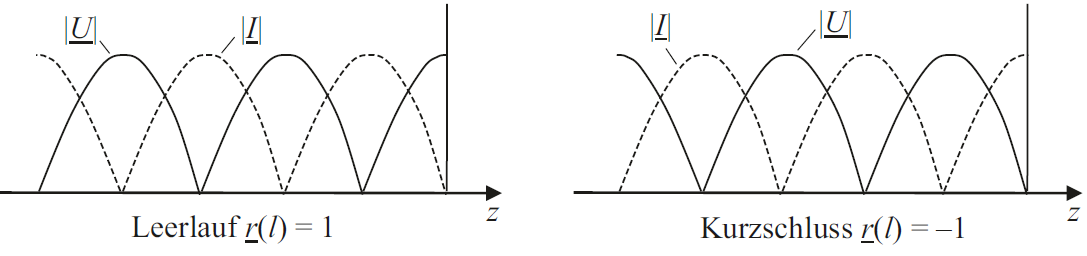
\includegraphics[width = \columnwidth]{images/Reflexion.png}

\subsection{Smith-Diagramm}
\begin{sectionbox}
    \[
        \underline{Z} = R + jX \hspace{7mm} \underline{Y} = G + jB = \frac{1}{\underline{Z}} = \frac{1}{R + jX} = \frac{R - jX}{R^2 + X^2}
    \]


    \textbf{Reflexionskoeffizient:}
    \[
        r = \frac{Z - Z_0}{Z + Z_0}
    \]

    \textbf{Leitungstransformation:}
    \[
        \underline{r}_A = \underline{r}_E \cdot e^{-j\beta l} \hspace{5mm} \text{mit} \hspace{5mm} \beta = \frac{2\pi}{\lambda}
    \]



    \textbf{Operationen im Smith-Diagramm:}
    \begin{itemize}
        \item Verlängern der (verlustlosen) Leitung: Drehung im Uhrzeigersinn um den Mittelpunkt
        \item Induktivität in Reihe schalten: Erhöhung von $X$, verringerung von $B$
        \item Kapazität in Reihe schalten: Verringerung von $X$, Erhöhung von $B$
        \item Induktivität parallel schalten: Verringerung von $X$, Erhöhung von $B$
        \item Kapazität parallel schalten: Erhöhung von $X$, Verringerung von $B$
    \end{itemize}

\end{sectionbox}

\section{S-Parameter}
\begin{sectionbox}
    \textbf{Streumatrix:}
    \[
        \setlength{\arraycolsep}{20pt}
        \begin{array}{cccc}
        S_{11} = \left. \frac{b_1}{a_1} \right|_{a_2 = 0} & 
        S_{12} = \left. \frac{b_1}{a_2} \right|_{a_1 = 0} \\[10pt]
        S_{21} = \left. \frac{b_2}{a_1} \right|_{a_2 = 0} &
        S_{22} = \left. \frac{b_2}{a_2} \right|_{a_1 = 0}
        \end{array}
    \]
    
    \begin{itemize}
        \item Reziprozität: $S_{12} = S_{21}$
        \item Symmetrie: $S_{11} = S_{22}$
        \item Verlustfreies Zweitor: $\vec{S}^T \cdot \vec{S}^* = \vec{I}$  bzw.  $|S_{21}|^2 = 1 - |S_{11}|^2$
    \end{itemize}
    
\end{sectionbox}
sd
\end{document}